\documentclass[10pt,aspectratio=43,mathserif,table]{beamer} 
%设置为 Beamer 文档类型,设置字体为 10pt,长宽比为16:9,数学字体为 serif 风格
\batchmode

\usepackage{graphicx}
\usepackage{animate}
\usepackage{hyperref}

%导入一些用到的宏包
\usepackage{amsmath,bm,amsfonts,amssymb,enumerate,epsfig,bbm,calc,color,ifthen,capt-of,multimedia,hyperref}
\usepackage{xeCJK} %导入中文包
\setCJKmainfont{SimHei} %字体采用黑体  Microsoft YaHei

\usetheme{Goettingen} %主题
%\usecolortheme{sustech} %主题颜色

\usepackage[ruled,linesnumbered]{algorithm2e}

\usepackage{fancybox}
\usepackage{xcolor}
\usepackage{times}
\usepackage{listings}

\usepackage{booktabs}
\usepackage{colortbl}

\newcommand{\Console}{Console}
\lstset{ %
	backgroundcolor=\color{white},   % choose the background color
	basicstyle=\footnotesize\rmfamily,     % size of fonts used for the code
	columns=fullflexible,
	breaklines=true,                 % automatic line breaking only at whitespace
	captionpos=b,                    % sets the caption-position to bottom
	tabsize=4,
	commentstyle=\color{mygreen},    % comment style
	escapeinside={\%*}{*)},          % if you want to add LaTeX within your code
	keywordstyle=\color{blue},       % keyword style
	stringstyle=\color{mymauve}\ttfamily,     % string literal style
	numbers=left, 
	%	frame=single,
	rulesepcolor=\color{red!20!green!20!blue!20},
	% identifierstyle=\color{red},
	language=c
}




\setsansfont{FangSong}
\setmainfont{FangSong}

\definecolor{mygreen}{rgb}{0,0.6,0}
\definecolor{mymauve}{rgb}{0.58,0,0.82}
\definecolor{mygray}{gray}{.9}
% \definecolor{mypink}{rgb}{.99,.91,.95}
\definecolor{mycyan}{cmyk}{.3,0,0,0}
\definecolor{mypink}{rgb}{1, 0.75, 0.8}


%题目,作者,学校,日期
\title{学术研究经验分享}
\subtitle{\fontsize{9pt}{14pt}\textbf{——从RA到Researcher}}
\author{汇报人:孟克}

\vspace{4em}

\institute{\fontsize{8pt}{14pt}对外经济贸易大学中国WTO研究院}
\date{\fontsize{6pt}{10pt}{2024.9.13}}

%学校Logo
%\pgfdeclareimage[height=0.5cm]{sustech-logo}{sustech-logo.png}
%\logo{\pgfuseimage{sustech-logo}\hspace*{0.3cm}}

\setbeamerfont{section title}{size=\normalsize}
\setbeamerfont{subsection title}{size=\small}


% -----------------------------------------------------------------------------
\begin{document}
% -----------------------------------------------------------------------------

\frame{\titlepage}

\section[目录]{}   %目录
\begin{frame}{目录}
\tableofcontents
\end{frame}

% -----------------------------------------------------------------------------
\section{1.培养环节关键节点与毕业要求}  %引言

\subsection{1.1 博士生4年培养总览}
\begin{frame}{\small 1.1 博士生4年培养总览}
	\begin{figure}[htbp]
		\centering
		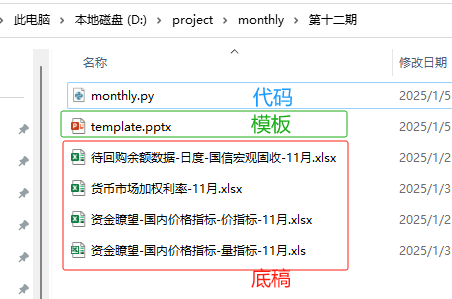
\includegraphics[width=0.85\textwidth]{figs/fig1.png}
		%\caption{图片标题}
		\label{fig:indicator}
	\end{figure}
\end{frame}

\subsection{1.2 毕业资格关键要点}
\begin{frame}{\small 1.2 毕业资格关键要点}
	\begin{block}{\footnotesize 学位申请关键点:}
		 \begin{itemize}
		 	\item \footnotesize \href{https://law.uibe.edu.cn/docs/2022-07/297b8754a81b460ea4cffecce1d491f4.pdf}{\textcolor{blue}{\underline{博士毕业资格}}}为: 1项一级成果,或2项二级成果,或3项三级成果
		 \end{itemize}
		 
		 \begin{itemize}
		 	\item \footnotesize 开题答辩前需要有与拟开题目相关的一篇论文(最好是C)
		 \end{itemize}
		 
		 \begin{itemize}
		 	\item \footnotesize 三年级下学期(6月)最后一次开题机会,如未能达标则意味着延毕
		 \end{itemize}
		 
		 \begin{itemize}
		 	\item \footnotesize 学位论文(大论文)要在保稳的基础上谈创新
		 \end{itemize}
	\end{block}
		
	
	\begin{block}{\footnotesize 学业考试关键点:}
		
		\begin{itemize}
			\item \footnotesize 三高尽量平时学好(尤其宏观),听不懂也不要焦虑,好好突击也能过
		\end{itemize}
		
		
		\begin{itemize}
			\item \footnotesize 重视理论学习,理论学习与学术研究是相辅相成的:
			\begin{itemize}
				\item \footnotesize 开始上课时或许听不太懂,但随着研究的深入会逐渐回归到理论中
			\end{itemize}
			\begin{itemize}
				\item \footnotesize 开始做研究时或无从下手,但对理论的学习有助于更好地认识研究
			\end{itemize}
		\end{itemize}
		
		\begin{itemize}
			\item \footnotesize 一年级做好笔记,为二年级的\href{https://yjsy.uibe.edu.cn/cms/infoSingleArticle.do?articleId=7172}{{\textcolor{blue}{\underline{博士资格考试(博资考)}}}}做准备
		\end{itemize}
		
		\begin{itemize}
			\item \footnotesize 博资考挂科率较高,尽量提早准备
		\end{itemize}
	\end{block}
\end{frame}




\section{2.博士研究生如何开展研究}  %引言

\subsection{2.1 何为好的研究?}
\begin{frame}{\small 2.1 何为好的研究?}
	
	\begin{block}{\footnotesize 一个好的研究可能包含以下要素:}
		\begin{itemize}
			\vspace{0.7em}
			\item \footnotesize 研究问题
			\begin{itemize}
				\item \footnotesize 有理论贡献(国内所缺少的),应站在已有文献的视角,讨论本文的理论贡献,提出或扩展新的理论框架 
			\end{itemize}
			
			\begin{itemize}
				\item \footnotesize 研究应有现实意义,面向实际问题,或提出新问题、新视角
			\end{itemize}
			
			\begin{itemize}
				\item \footnotesize 研究问题要清晰明确,避免模糊,帮助精确设计研究
			\end{itemize}
			
			%%%%%%%%%%%%%%%%%%%%%%%%%%%%%%%%%%%%%%%%%
			\vspace{0.7em}
			\item \footnotesize 研究方法
			
			\begin{itemize}
				\item \footnotesize 模型构建合理,实证模型或理论模型逻辑严密,假设合理
			\end{itemize}
			
			\begin{itemize}
				\item \footnotesize 重视因果推断(Causal Inference),Model-Based 转向 Design-Based,使用合适的工具(DID、Bartik-IV、RD)
			\end{itemize}
			
			\begin{itemize}
				\item \footnotesize 数据使用准确可靠,数据典型事实不可违背现实
			\end{itemize}
			
			%%%%%%%%%%%%%%%%%%%%%%%%%%%%%%%%%%%%%%%%%
			\vspace{0.7em}
			\item \footnotesize 研究贡献
			
			\begin{itemize}
				\item \footnotesize 确保研究问题的长期价值(可持续性、持久性)
			\end{itemize}
			
			\begin{itemize}
				\item \footnotesize 跨学科视角的融入
			\end{itemize}
		
		\end{itemize}
	\end{block}
	
\end{frame}



\subsection{2.2 怎样才能做出好的研究?}
\begin{frame}{\small 2.2 怎样才能做出好的研究?}
	
	\begin{block}{\footnotesize 学术sense的养成,要注意:}
		\vspace{0.7em}
		
		\begin{itemize}
			\item \footnotesize 要对经济学前沿文献有所认知
			
			\begin{itemize}
				\item \footnotesize 养成读文献的好习惯,target on TOP 5,多读top-tier外文
			\end{itemize}
			
			\begin{itemize}
				\item \footnotesize 读文献时,重点关注Introduction和Identification
			\end{itemize}
			
			\begin{itemize}
				\item \footnotesize 不要固步自封,万万不可仅把眼光局限于自己所谓的研究领域
			\end{itemize}
			
			\begin{itemize}
				\item \footnotesize 结合文献进行深度思考
			\end{itemize}
			
			\vspace{0.7em}
			%%%%%%%%%%%%%%%%%%%%%%%%%%%%%%%%%%%%%%%%%
			
			\item \footnotesize 要熟练掌握经济学研究方法
			
			\begin{itemize}
				\item \footnotesize 简约式估计(reduced form)or  结构式估计(structural-form)
			\end{itemize}
			
			\begin{itemize}
				\item \footnotesize 学会如何做好实证设计,学会做好的因果识别
			\end{itemize}
				
			

			\vspace{0.7em}
			%%%%%%%%%%%%%%%%%%%%%%%%%%%%%%%%%%%%%%%%%
			
			\item \footnotesize 不要唯成果论,对“好期刊”“优秀学长学姐”甚至“老师”祛魅,凡事要问“Why?”和“So?”(当然是要经过思考且有依据的,而不是抬杠)
			
			
			
			\vspace{0.7em}
			%%%%%%%%%%%%%%%%%%%%%%%%%%%%%%%%%%%%%%%%%
			
			\item \footnotesize 保持阅读,多思考,勤动手
			

			
		\end{itemize}
	\end{block}
	
\end{frame}


\subsection{2.3 学术入门做RA!}
\begin{frame}{\small 2.3 学术入门做RA!}
	
	\begin{block}{\footnotesize 从RA做起,切勿好高骛远(博一-博三):}
		\begin{itemize}
			\item \footnotesize RA(researcher assistance),是指在学术或研究项目中,辅助研究人员(导师、副导师)完成研究任务的角色。做好RA是实现干中学自我提升最快的阶段
			\vspace{0.4em}
			\begin{itemize}
				\item \footnotesize 理论深化:广泛阅读文献,深入了解研究领域
			\end{itemize}
			\vspace{0.4em}
			\begin{itemize}
				\item \footnotesize 研究技能:掌握文献查阅、数据分析、写作的完整流程
			\end{itemize}
			\vspace{0.4em}
			\begin{itemize}
				\item \footnotesize 数据分析:熟练使用统计或编程语言(如Stata、R、Python)
			\end{itemize}
			\vspace{0.4em}
			\begin{itemize}
				\item \footnotesize 批判性思维:评估文献,质疑假设,培养独立思考能力
			\end{itemize}
			\vspace{0.4em}
			\begin{itemize}
				\item \footnotesize 写作与表达:锻炼学术写作,清晰传达复杂理论和结果
			\end{itemize}
			\vspace{0.4em}
			\begin{itemize}
				\item \footnotesize 时间管理:同时处理数据、文献、写作,培养多任务管理能力
			\end{itemize}
			\vspace{0.4em}
			\begin{itemize}
				\item \footnotesize 团队协作:提高沟通技巧,学习汇报进展、讨论问题和接受反馈
			\end{itemize}
			\vspace{0.4em}
			\begin{itemize}
				\item \footnotesize 研究兴趣探索:帮助确定学术兴趣,打下博士论文选题基础
			\end{itemize}
			
		\end{itemize}
	\end{block}
	
\end{frame}



\subsection{2.4 培养独立科研的能力,成为researcher}
\begin{frame}{\small 2.4 培养独立科研的能力,成为researcher}
	
	\begin{block}{\footnotesize 从RA到Researcher的角色转变(博三-博四):}
	\begin{itemize}
		\item \footnotesize RA:作为助理,辅助导师完成科研任务,主要执行具体的任务
		\vspace{0.4em}
		\begin{itemize}
			\item \footnotesize 任务导向:负责文献查阅、数据处理、撰写部分报告,依赖导师指导
		\end{itemize}
		\vspace{0.4em}
		\begin{itemize}
			\item \footnotesize 技术支持:掌握数据分析工具和基础研究技能,执行具体的研究步骤
		\end{itemize}
		\vspace{0.9em}
		
		\item \footnotesize Researcher:能够独立提出问题、设计研究并完成整个科研流程
		\vspace{0.4em}
		\begin{itemize}
			\item \footnotesize 问题提出:涉及研究,自主设计研究计划并提出命题
		\end{itemize}
		\vspace{0.4em}
		\begin{itemize}
			\item \footnotesize 独立性:从数据收集、分析到撰写与发表,独立完成研究项目
		\end{itemize}
		\vspace{0.4em}
		\begin{itemize}
			\item \footnotesize 学术领导力:在团队中起局部领导作用,推动科研并指导他人
		\end{itemize}
		\vspace{0.4em}
		
	\end{itemize}
\end{block}
	
\end{frame}




\section{3.以积极心态迎接博士之旅}  %引言
\subsection{3.1 一个衡量博士生产出水平的量化模型}
\begin{frame}{\small 3.1 一个衡量博士生产出水平的量化模型}
	$$
	\small f(T, S, E, A, L) = \left( T^{\alpha} \cdot S^{\beta} \cdot E^{\gamma} \cdot A^{\delta} \right) \cdot (1 + kL)
	$$
	
	\small 其中:
	\begin{itemize}
		\item \footnotesize $T$: 导师的影响
		\item \footnotesize $S$: 学校平台的资源
		\item \footnotesize $E$: 学生的努力程度
		\item \footnotesize $A$: 学生的天赋
		\item \footnotesize $L$: 运气因素
		\item \footnotesize $\alpha, \beta, \gamma, \delta$: 各参数的权重,反映其对成功的影响大小
		\item \footnotesize $k$: 运气影响的系数
	\end{itemize}
	
	\vspace{2em}
	
	\small A possible specification:
	$$
	\small f(T, S, E, A, L) = \left( T^{0.4} \cdot S^{0.1} \cdot E^{0.25} \cdot A^{0.15} \right) \cdot L
	$$
\end{frame}



\subsection{3.2 如何缓解压力}
\begin{frame}{\small 3.2 如何缓解压力}
	
	\begin{block}{\footnotesize 不要有休息羞耻:}
		\begin{itemize}
			\item \footnotesize 博士生没做完工作也可以休息,只要心里有数,不拖ddl
		\end{itemize}
		\vspace{0.4em}
		
		\begin{itemize}
			\item \footnotesize 不必做组内最靠谱的人,不必老师随叫随到,导致自身精神紧绷
		\end{itemize}
		\vspace{0.4em}
	\end{block}
	
	
	\begin{block}{\footnotesize 理智的自我劝解,或与朋友老师交流:}
		
		\begin{itemize}
			\item \footnotesize 保持理智,做正确的选择,努力让自己内核稳定
		\end{itemize}
		\vspace{0.4em}		
		
		\begin{itemize}
			\item \footnotesize 情绪不要积压,很多事情的确是不吐不快
		\end{itemize}
		\vspace{0.4em}
		
	\end{block}
	
	
	\begin{block}{\footnotesize 培养兴趣爱好:}
		
		\begin{itemize}
			\item \footnotesize 最好是外向型爱好,例如打球、徒步
		\end{itemize}
		\vspace{0.4em}		
		
	\end{block}
	
\end{frame}



\subsection{3.3 如何与导师相处}
\begin{frame}{\small 3.3 如何与导师相处}
	
	\begin{itemize}
		\item \footnotesize 件件有着落,事事有回应,不拖沓
	\end{itemize}
	\vspace{0.4em}
		
	\begin{itemize}
		\item \footnotesize 遇事与导师沟通,拒绝情绪内耗
	\end{itemize}
	\vspace{0.4em}
	
	\begin{itemize}
		\item \footnotesize 找到自身价值,勇敢鉴定有信心
	\end{itemize}
	\vspace{0.4em}
	
	\begin{itemize}
		\item \footnotesize 导师说的也不一定对
	\end{itemize}
	\vspace{0.4em}
	
\end{frame}



\section{4.资料分享}  

\begin{frame}{\small 4.资料分享}
	
\begin{block}{\footnotesize 三高:}
		\vspace{-0.9em}
	\begin{minipage}[b]{0.4\textwidth} % 左边的文字部分占45%的宽度,底部对齐
		\begin{itemize}
			\item \footnotesize \href{https://pan.quark.cn/s/02f00a7a805a}{\textcolor{blue}{\underline{高级宏观笔记\&习题}}}
		\end{itemize}
		\vspace{0.4em}
		
		\begin{itemize}
			\item \footnotesize \href{https://pan.quark.cn/s/6decfec169e9}{\textcolor{blue}{\underline{高级微观笔记\&习题}}}
		\end{itemize}
		\vspace{0.4em}
		
		\begin{itemize}
			\item \footnotesize \href{https://pan.quark.cn/s/40b4626268ac}{\textcolor{blue}{\underline{高级计量笔记\&习题}}}
		\end{itemize}
		\vspace{0.4em}
	\end{minipage}
	\hfill
	\begin{minipage}[b]{0.55\textwidth} % 右边的图片部分占50%的宽度,底部对齐
		\centering
		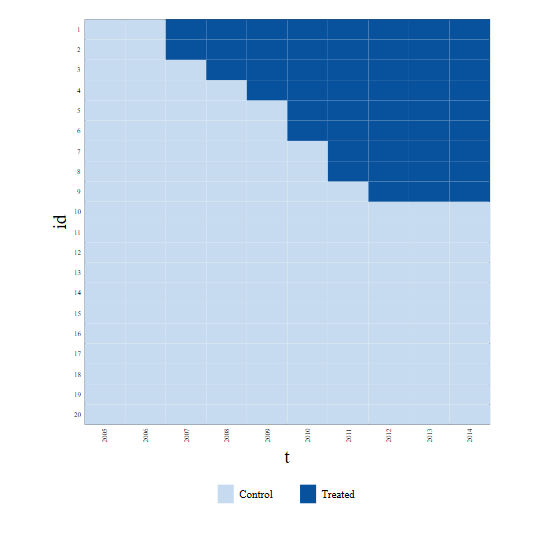
\includegraphics[width=\textwidth]{figs/fig2.png}
		%\caption{图片标题}
	\end{minipage}
	
	
\end{block}
	
\begin{block}{\footnotesize My info:}
	\vspace{1.5em}
	\begin{minipage}[b]{0.55\textwidth} % 左边的文字部分占55%的宽度,底部对齐
		      
		
		\begin{itemize}
			\item \footnotesize Blog:\quad \quad \href{https://mengke25.github.io}{\textcolor{blue}{\underline{mengke25.github.io}}}
		\end{itemize}
		\vspace{0.4em}    
		
		\begin{itemize}
			\item \footnotesize Github:\quad  \href{https://github.com/mengke25}{\textcolor{blue}{\underline{@mengke25}}}
		\end{itemize}
		\vspace{0.4em}    
	\end{minipage}
	\hfill
	\begin{minipage}[b]{0.2\textwidth} % 右边的图片部分占40%的宽度,底部对齐
		\centering
		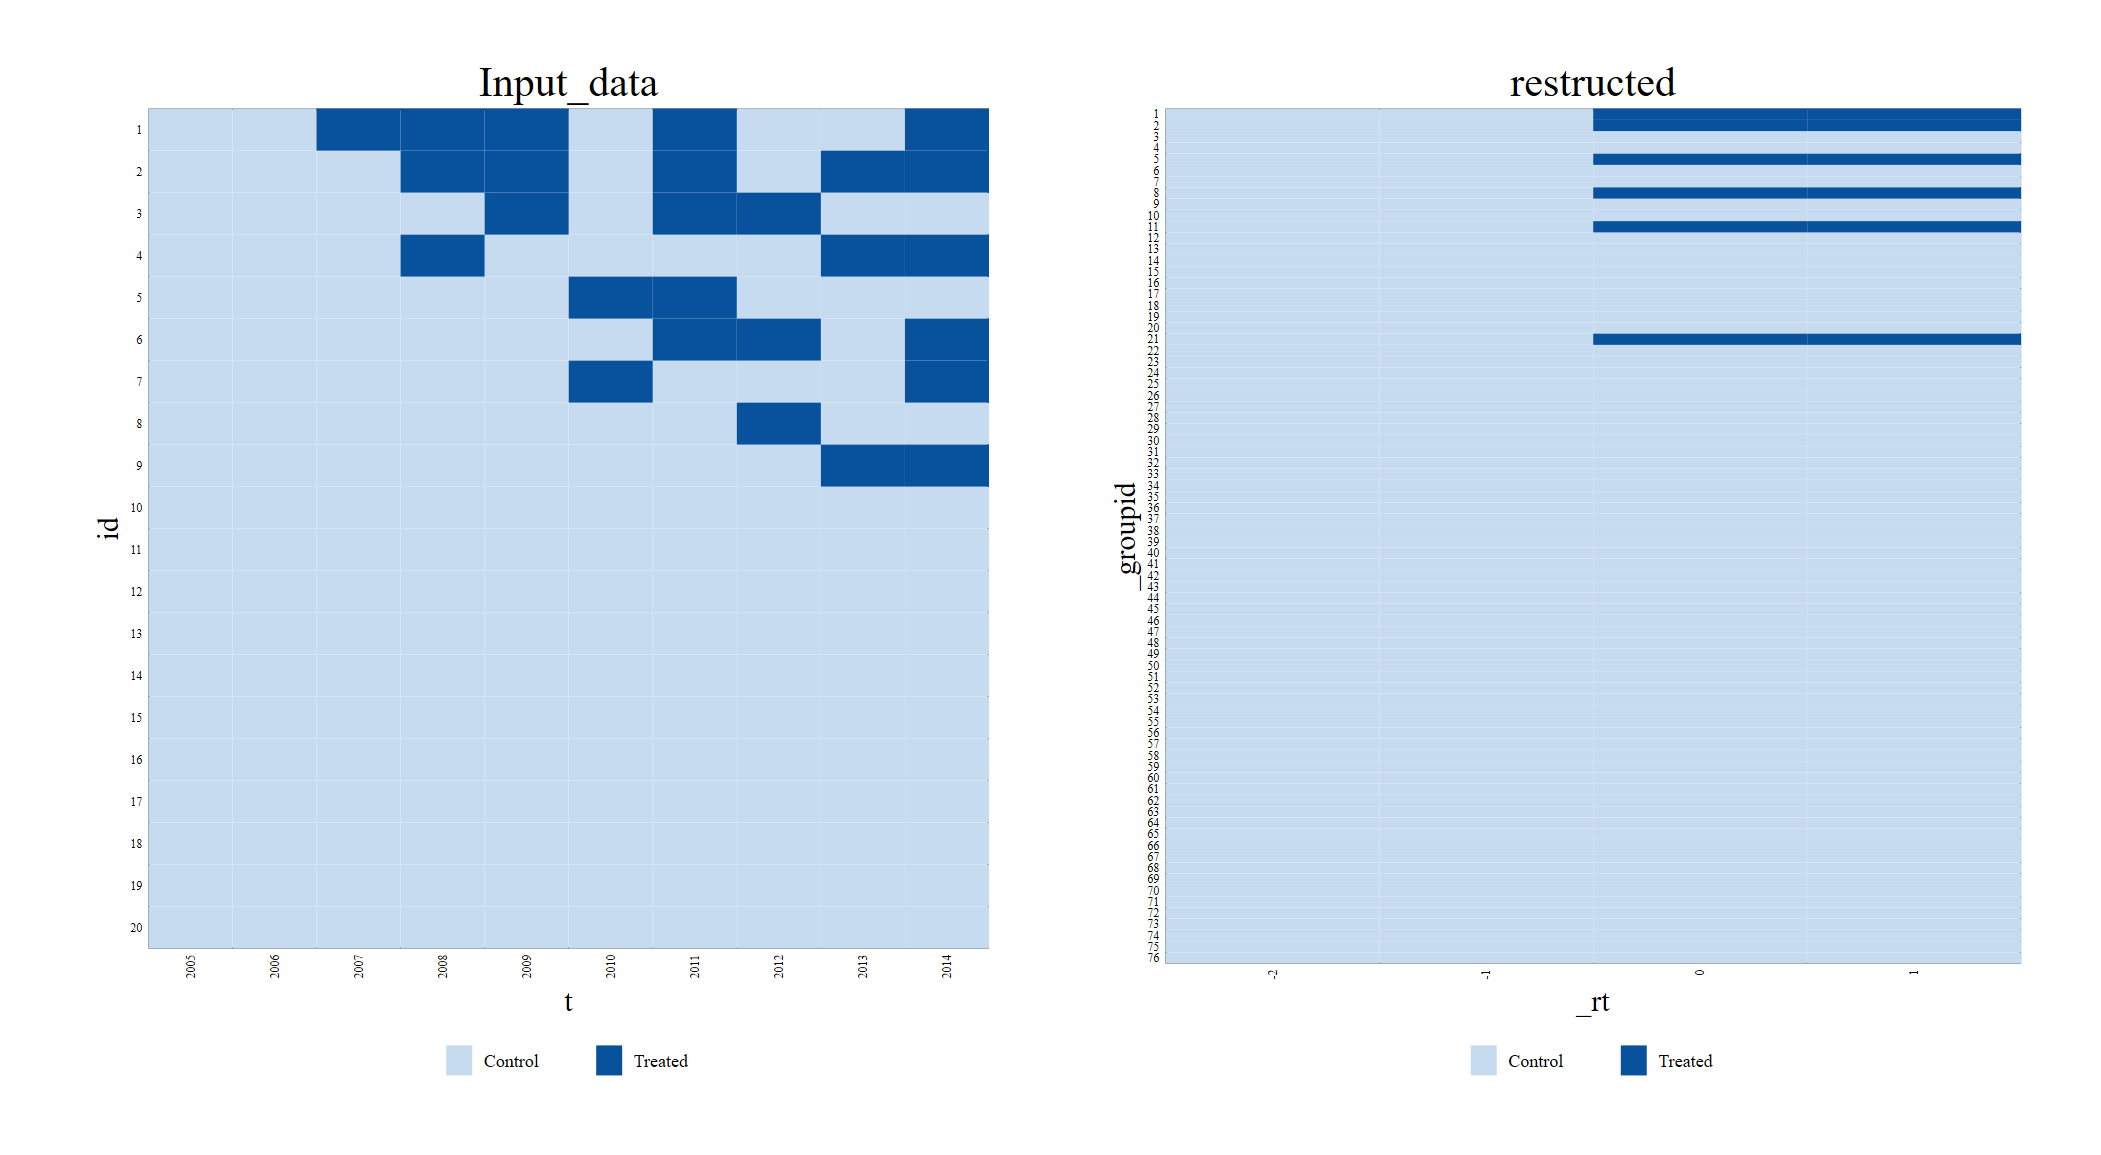
\includegraphics[width=\textwidth]{figs/fig4.png}
		%\caption{图片标题}
	\end{minipage}
\end{block}

\end{frame}



	
%\end{frame}

\end{document}